\documentclass[./../main.tex]{subfiles}
\graphicspath{{img/}}

\begin{document}
    \begin{exercise}[Primeros estados excitados del átomo de helio]
        Calcula la energía, a primer orden de aproximación, de los estados excitados del átomo de helio \(2^{1}S\), \(2^{1}P\), \(2^{3}S\) y \(2^{3}P\). Para hacer este cálculo será necesario obtener explícitamente las integrales de COulomb y de intercambio, \(J_{n\ell}\) y \(K_{n\ell}\) respectivamente. Recuerda que en clase vimos que las energías corregidas están dadas por la expresión

        \begin{equation}
            E_{n\ell,\pm} = E_{1n}^{(0)} + E_{n\ell,\pm}^{(1)} = -\dfrac{Z^{2}}{2}\left(1 + \dfrac{1}{n^{2}}\right) + J_{n\ell} \pm K_{n\ell}.
            \label{eq:energy-correction}
        \end{equation}

        Los niveles de energía quedaban como se ilustra en la siguiente figura:

        \begin{figure}[htb]
            \centering
            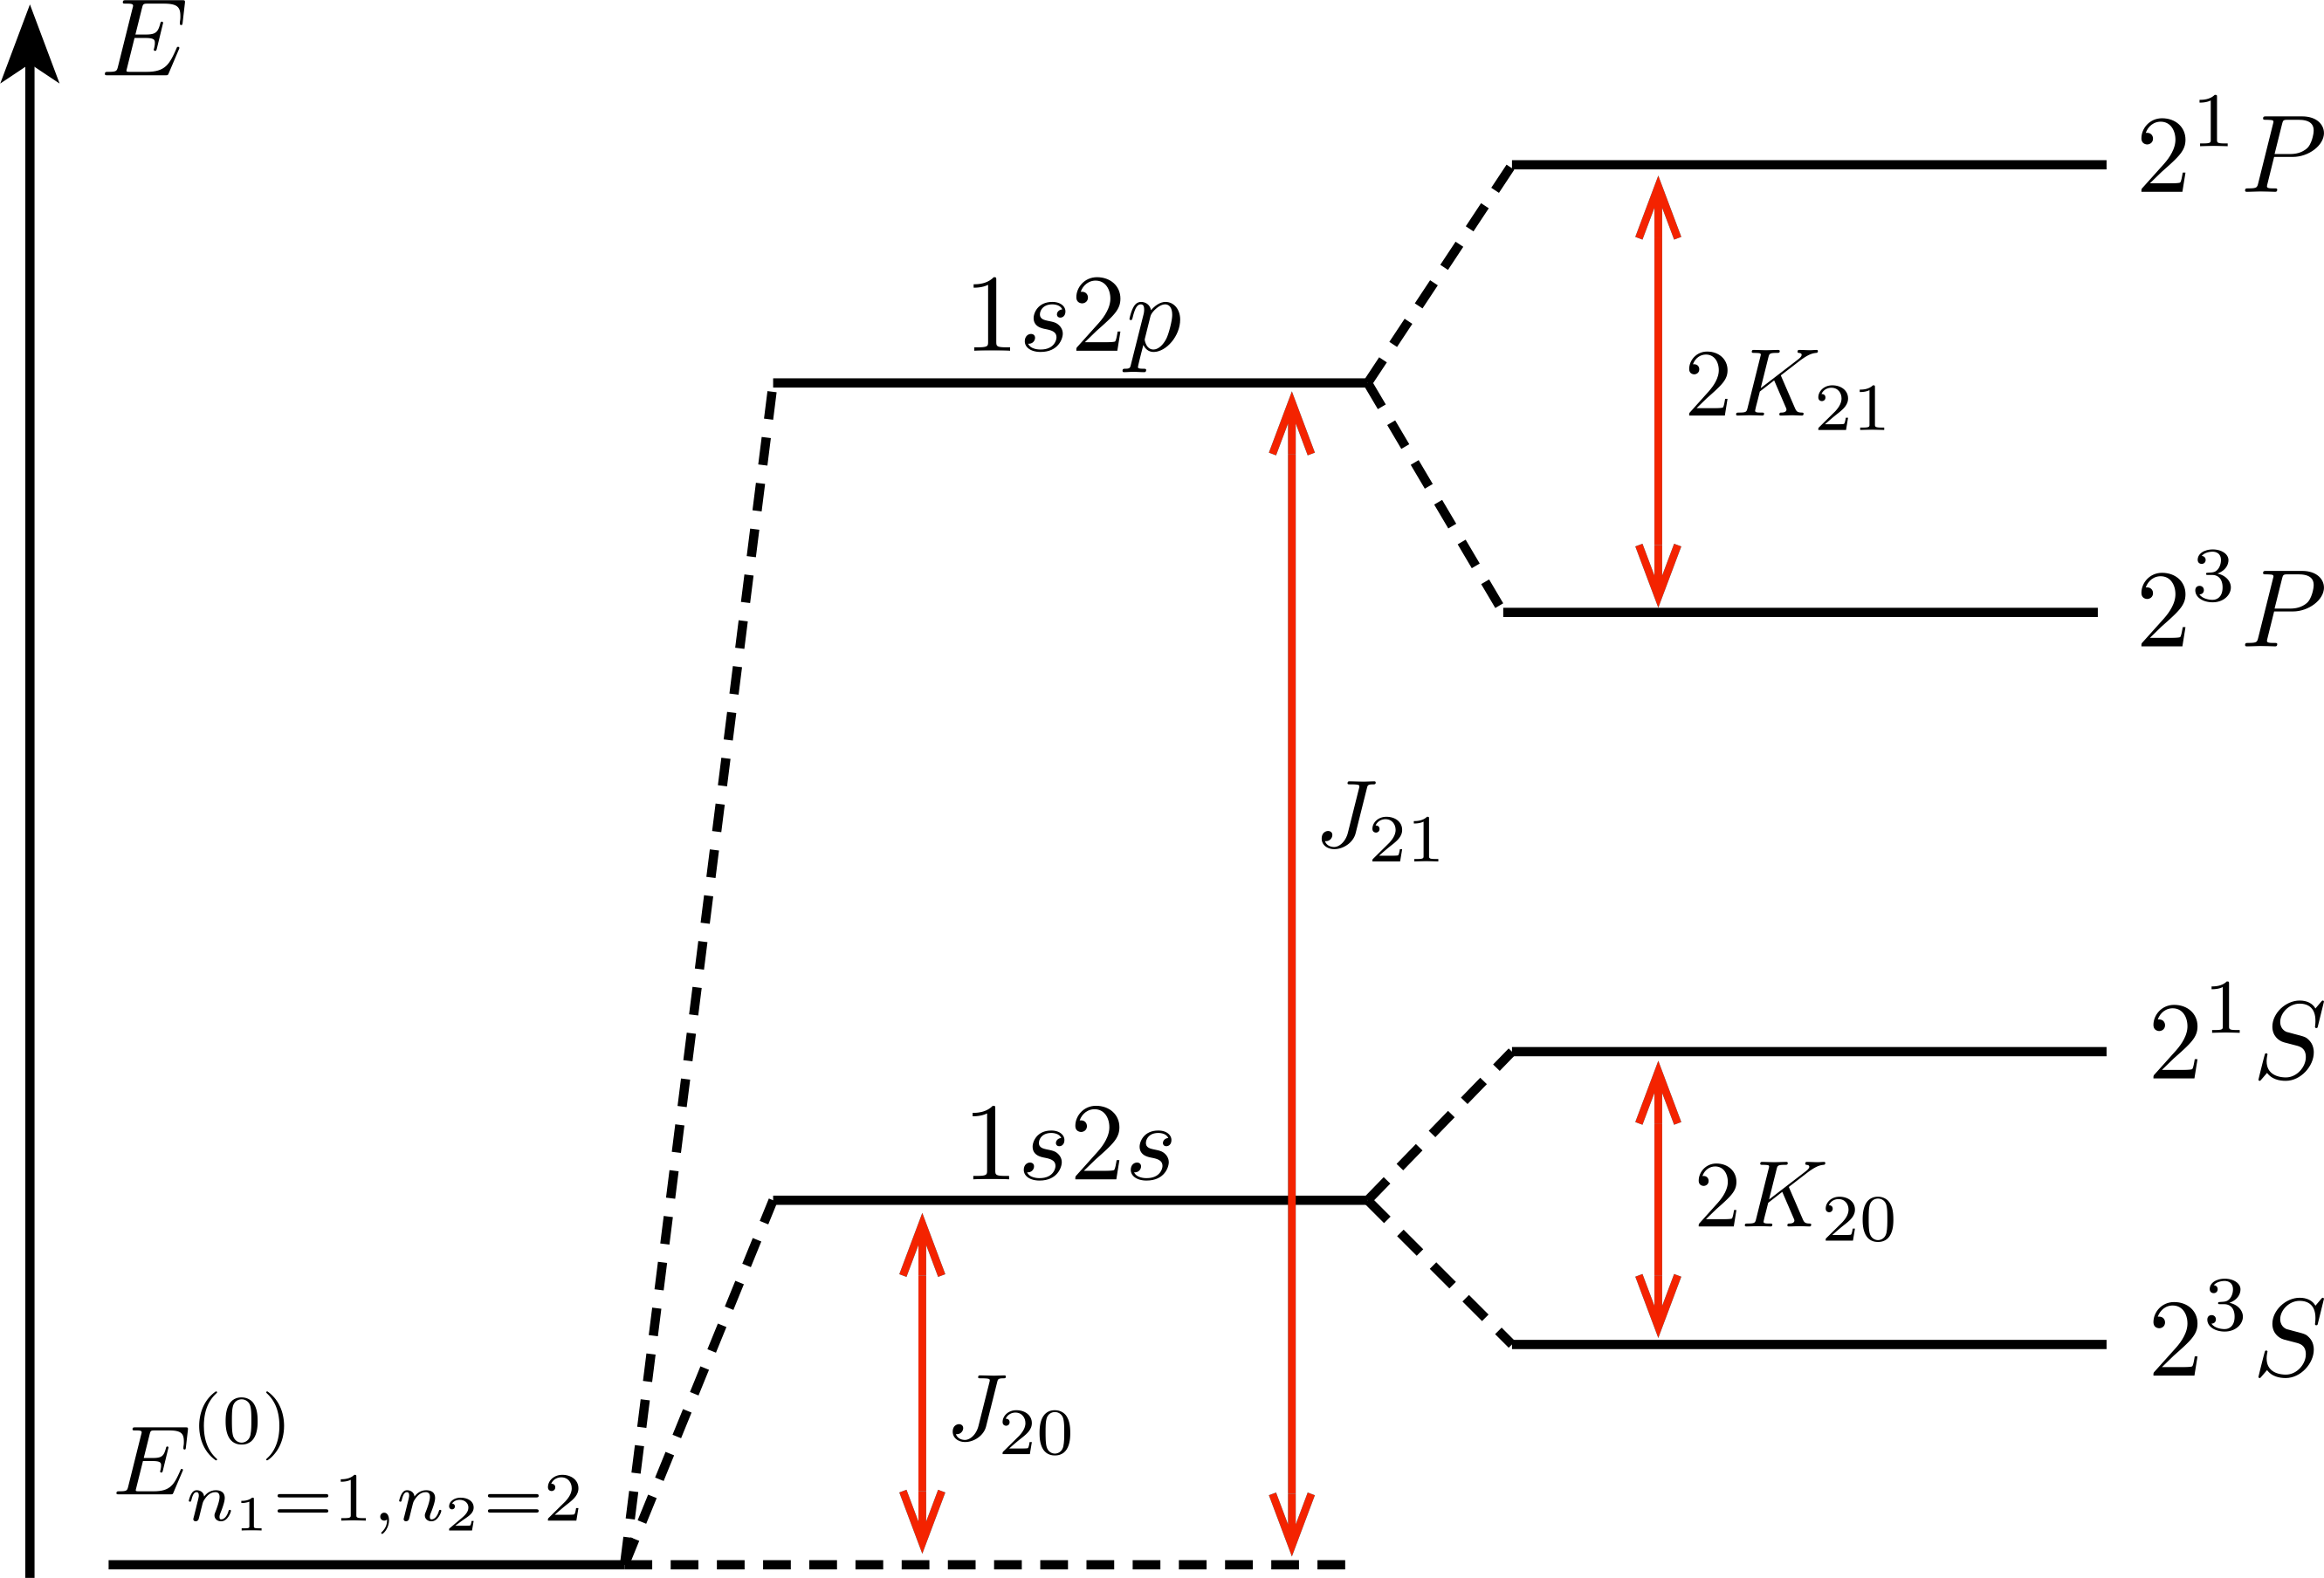
\includegraphics{first-excited-states}
            \caption{Primeros estados excitados del átomo de dos electrones.}
            \label{fig:first-excites-states-helium}
        \end{figure}

        \textbf{Nota importante:} Para resolver este ejercicio puedes usar directamente las integrales que se encontraron en clase para \(J_{n\ell}\) y \(K_{n\ell}\). Sin embargo, recuerda que éstas quedaban en términos de las variables \(r_{<}\) y \(r_{>}\). Es necesario que expliques con claridad cómo es que estas dos variables se emplean en el cálculo de las integrales, de manera que encuentres una expresión en términos ya no de \(r_{<}\) y \(r_{>}\), sino de \(r_{1}\) y \(r_{2}\) (\idest la coordenada radial de cada electrón). Una vez que hayas dejado este punto claro, las integrales que quedan pueden resolver a mano, o bien, usando cualquier software para hacer la integración. Si decides usar un software, es necesario que especifiques qué programa usaste y que anexes el código al ejercicio.

        \begin{solution}
            Debemos calcular la energía para los estados cuyo cuántico es \(n = 2\), tal que para \(\ell = 0\) los estados son \(2^{1}S\) y \(2^{3}S\), mientras que para \(\ell = 1\) los estados son \(2^{1}P\) y \(2^{3}P\). Las integrales a calcular son \(J_{20},J_{21}\) y \(K_{20},K_{21}\). \(J_{n\ell}\) y \(K_{n\ell}\), respectivamente, están dadas por las siguientes expresiones:

            \begin{align}
                J_{n\ell} &= \int_{0}^{\infty}\odif{r_{2}}r_{2}^{2}R_{n\ell}^{2}(r_{2})\int_{0}^{\infty}\odif{r_{1}}r_{1}^{2}R_{10}^{2}(r_{1})\dfrac{1}{r_{>}},\label{eq:CoulombIntegral}\\
                K_{n\ell} &= \dfrac{1}{2\ell + 1}\int_{0}^{\infty}\odif{r_{2}}r_{2}^{2}R_{10}(r_{2})R_{n\ell}(r_{2})\int_{0}^{\infty}\odif{r_{1}}r_{1}^{2}R_{10}(r_{1})R_{n\ell}(r_{1})\dfrac{(r_{<})^{\ell}}{(r_{>})^{\ell + 1}}.\label{eq:ExchangeIntegral}
            \end{align}

            Sin embargo, notamos que están en términos de \(r_{<}\) y \(r_{>}\), por lo que debemos \emph{deshacernos} de estas variables, lo cual se logra integrando por intervalos. Recordando que

            \begin{align*}
                r_{<} &\implies \text{menor entre}\; r_{1}\;\text{y}\; r_{2},\\
                r_{>} &\implies \text{mayor entre}\; r_{1}\;\text{y}\; r_{2}.
            \end{align*}

            Entonces, integrando por intervalos, \(0 \leq r_{1} \leq r_{2}\) y \(r_{2} \leq r_{1} < \infty\), \cref{eq:CoulombIntegral} queda como

            \begin{equation}
                J_{n\ell} = \int_{0}^{\infty}\odif{r_{2}}r_{2}^{2}R_{n\ell}^{2}(r_{2})\left\lbrace\int_{0}^{r_{2}}\odif{r_{1}}r_{1}^{2}R_{10}^{2}(r_{1})\cdot\dfrac{1}{r_{2}} + \int_{r_{2}}^{\infty}\odif{r_{1}}r_{1}^{2}R_{10}^{2}(r_{1})\cdot\dfrac{1}{r_{1}}\right\rbrace.
                \label{eq:CoulombIntegralIntervals}
            \end{equation}

            De manera similar, \cref{eq:ExchangeIntegral} queda como

            \begin{equation}
                K_{n\ell} = 
                \begin{multlined}[t]
                    \int_{0}^{\infty}\odif{r_{2}}r_{2}^{2}R_{10}(r_{2})R_{n\ell}(r_{2})\mul\\
                    \mul\left\lbrace\int_{0}^{r_{2}}\odif{r_{1}}r_{1}^{2}R_{10}(r_{1})R_{n\ell}(r_{1})\cdot\dfrac{(r_{1})^{\ell}}{(r_{2})^{\ell + 1}} + \int_{r_{2}}^{\infty}\odif{r_{1}}r_{1}^{2}R_{10}(r_{1})R_{n\ell}(r_{1})\cdot\dfrac{(r_{2})^{\ell}}{(r_{1})^{\ell + 1}}\right\rbrace.    
                \end{multlined}
                \label{eq:ExchangeIntegralIntervals}
            \end{equation}

            Las funciones de onda radiales útiles, considerando unidades atómicas, son:

            \begin{align*}
                R_{10}(r) &= 2Z^{\slashfrac{3}{2}}\exp\left(-Zr\right),\\
                R_{20}(r) &= 2\left(\dfrac{Z}{2}\right)^{\slashfrac{3}{2}}\left(1 - \dfrac{Zr}{2}\right)\exp\left(-\dfrac{Zr}{2}\right),\\
                R_{21}(r) &= \dfrac{Zr}{\sqrt{3}}\left(\dfrac{Z}{2}\right)^{\slashfrac{3}{2}}\exp\left(-\dfrac{Zr}{2}\right).
            \end{align*}

            El programa que se utilizó para calcular las integrales fue \texttt{Mathematica} y al final del ejercicio se anexa el código.

            \pagebreak
            A partir de estas funciones de onda radiales, así como de \cref{eq:CoulombIntegralIntervals,eq:ExchangeIntegralIntervals} calculamos las integrales para los estados con \(n = 2\) y \(\ell = 0\),

            \begin{empheq}[box = \resultbox]{equation}
                \begin{aligned}
                    J_{20} &= \dfrac{34}{81},\\
                    K_{20} &= -\dfrac{32}{729}.
                \end{aligned}
                \label{eq:J20K20}
            \end{empheq}

            Y para los estados con \(n = 2\) y \(\ell = 1\),

            \begin{empheq}[box = \resultbox]{equation}
                \begin{aligned}
                    J_{21} &= \dfrac{118}{243},\\
                    K_{21} &= \dfrac{224}{6561}.
                \end{aligned}
                \label{eq:J21K21}
            \end{empheq}

            Por lo que de \cref{eq:J20K20}, la corrección a primer orden para los estados \(2^{1}S\) y \(2^{3}S\) es

            \begin{empheq}[box=\resultbox]{equation}
                E_{20,\pm}^{(1)} = \dfrac{34}{81} \pm \dfrac{32}{729}.
                \label{eq:FirstOrderCorrectionS}
            \end{empheq}

            Y de \cref{eq:J21K21}, la corrección a primer orden para los estados \(2^{1}P\) y \(2^{3}P\) es

            \begin{empheq}[box=\resultbox]{equation}
                E_{21,\pm}^{(1)} = \dfrac{118}{243} \pm \dfrac{224}{6561}.
                \label{eq:FirstOrderCorrectionP}
            \end{empheq}

            Mientras que la energía imperturbada es

            \begin{align}
                E_{12}^{(0)} &= -\dfrac{2^{2}}{2}\left(1 + \dfrac{1}{2^{2}}\right)\nonumber\\
                \Aboxedmain{E_{12}^{(0)} &= -\dfrac{5}{2}.}\label{eq:UnperturbedEnergy}
            \end{align}

            Por lo que la energía corregida a primer order, \cref{eq:energy-correction}, para los estados \(2^{1}S\) y \(2^{3}S\) es

            \begin{empheq}[box=\resultbox]{equation*}
                E_{20,\pm} = -\dfrac{5}{2} + \left(\dfrac{34}{81} \pm \dfrac{32}{729}\right).
            \end{empheq}

            Y, para los estados \(2^{1}P\) y \(2^{3}P\), es

            \begin{empheq}[box=\resultbox]{equation*}
                E_{21,\pm} = -\dfrac{5}{2} + \left(\dfrac{118}{243} \pm \dfrac{224}{6561}\right).
            \end{empheq}

            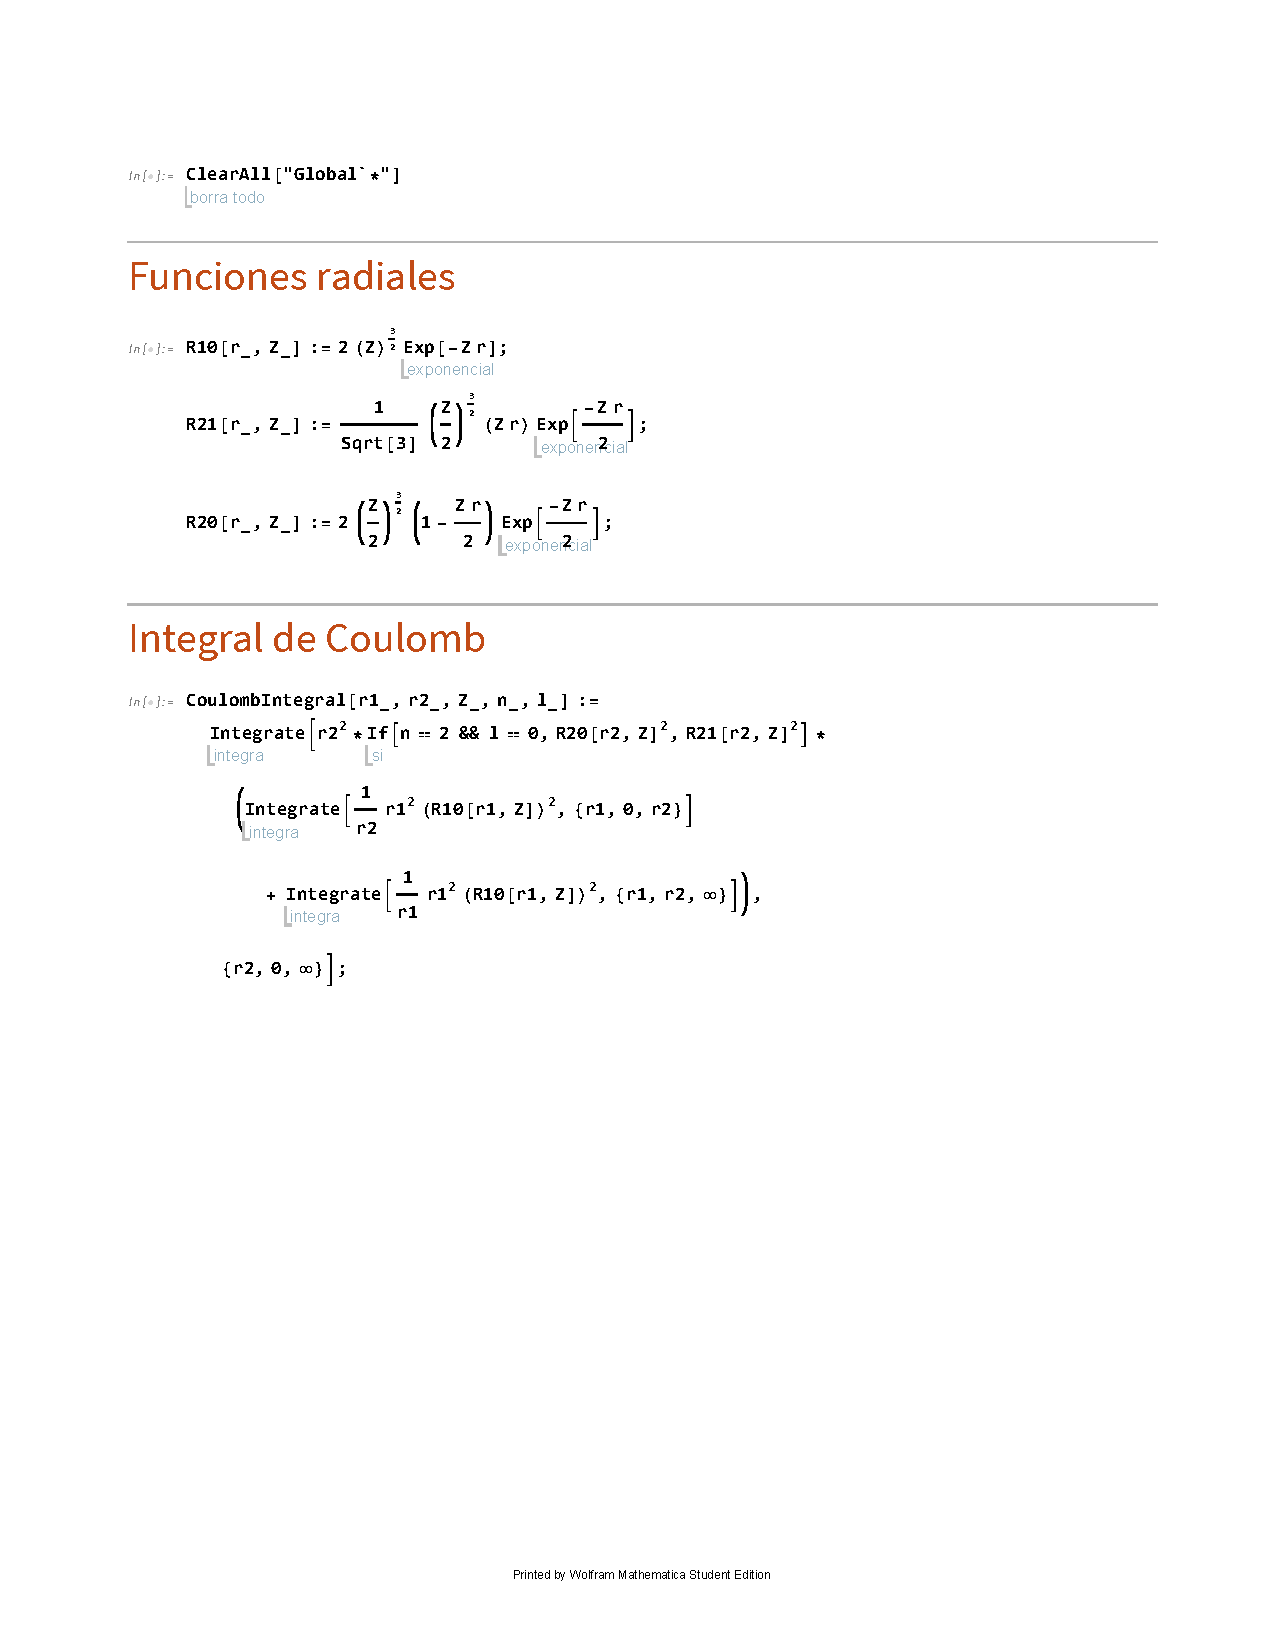
\includepdf[pages={1-3},pagecommand={\thispagestyle{fancy}},width=1.2\textwidth, trim={0 2cm 0 2cm}, clip]{../integrals.pdf}
            % \hspace*{-0.7cm}\includegraphics[page=4, trim={1.95cm 22cm 0 3cm}, width=\linewidth, clip]{../integrals.pdf}
        \end{solution}
    \end{exercise}
\end{document}